\subsection{Problem statement}
\label{subsec:problem-statement}

The Discovery~\footnote{\url{https://discovery.ic.unicamp.br/}} laboratory, located at \ac{UNICAMP}~\footnote{\url{https://ic.unicamp.br/}}, is working on a seismic analysis project with Petrobras~\footnote{\url{https://petrobras.com.br/}}.
\EBRP{This project relies heavily on machine learning and seismic operators for its computing graphs.}{This project aims at developing a framework to facilitate the execution of machine learning algorithms and seismic attribute operators on computing clusters.}
However, the input of these graphs is a massive seismic dataset that can contain terabytes of data.
Even supercomputers do not have enough memory to handle the computation on a single node.
Therefore, usually the execution is distributed by using data parallelism.

To facilitate this process, our laboratory implemented a framework called \ac{DASF}~\cite{dasf} that simplifies the development of data-parallel computing graphs using Dask~\cite{dask} under the hood.
\ac{DASF}~\cite{dasf} has an input parameter called \textbf{block\_size} that defines the size of each seismic block used during data parallelism.
However, setting this parameter can be challenging because it required finding the optimal relationship between it and the network overhead caused by it.

To illustrate this challenge, I present image~\ref{fig:block-size} which contains three computing graphs receiving input data from a seismic dataset.
The first graph \EBRP{shows the}{illustrates the situation in which the} input data \EBRP{as the entire dataset}{is processed as a whole}, which requires a significant amount of memory to \EBRP{execute}{store the data during the execution}.
The second graph divides the data into thousands of small parts, reducing the memory requirements but adding \EBRP{network overhead}{extra overhead on the network and the scheduler}.
\EB{Daniel, não está claro para mim se a sobrecarga de desempenho vem do scheduler ou da rede - você tem insights sobre isso?}
The third graph divides the data into a smaller number of parts, minimizing both network and memory requirements.

\begin{figure}[ht]
  \caption{Block size impact on memory and network usage}
  \label{fig:block-size}
  \resizebox{\textwidth}{!}{%
    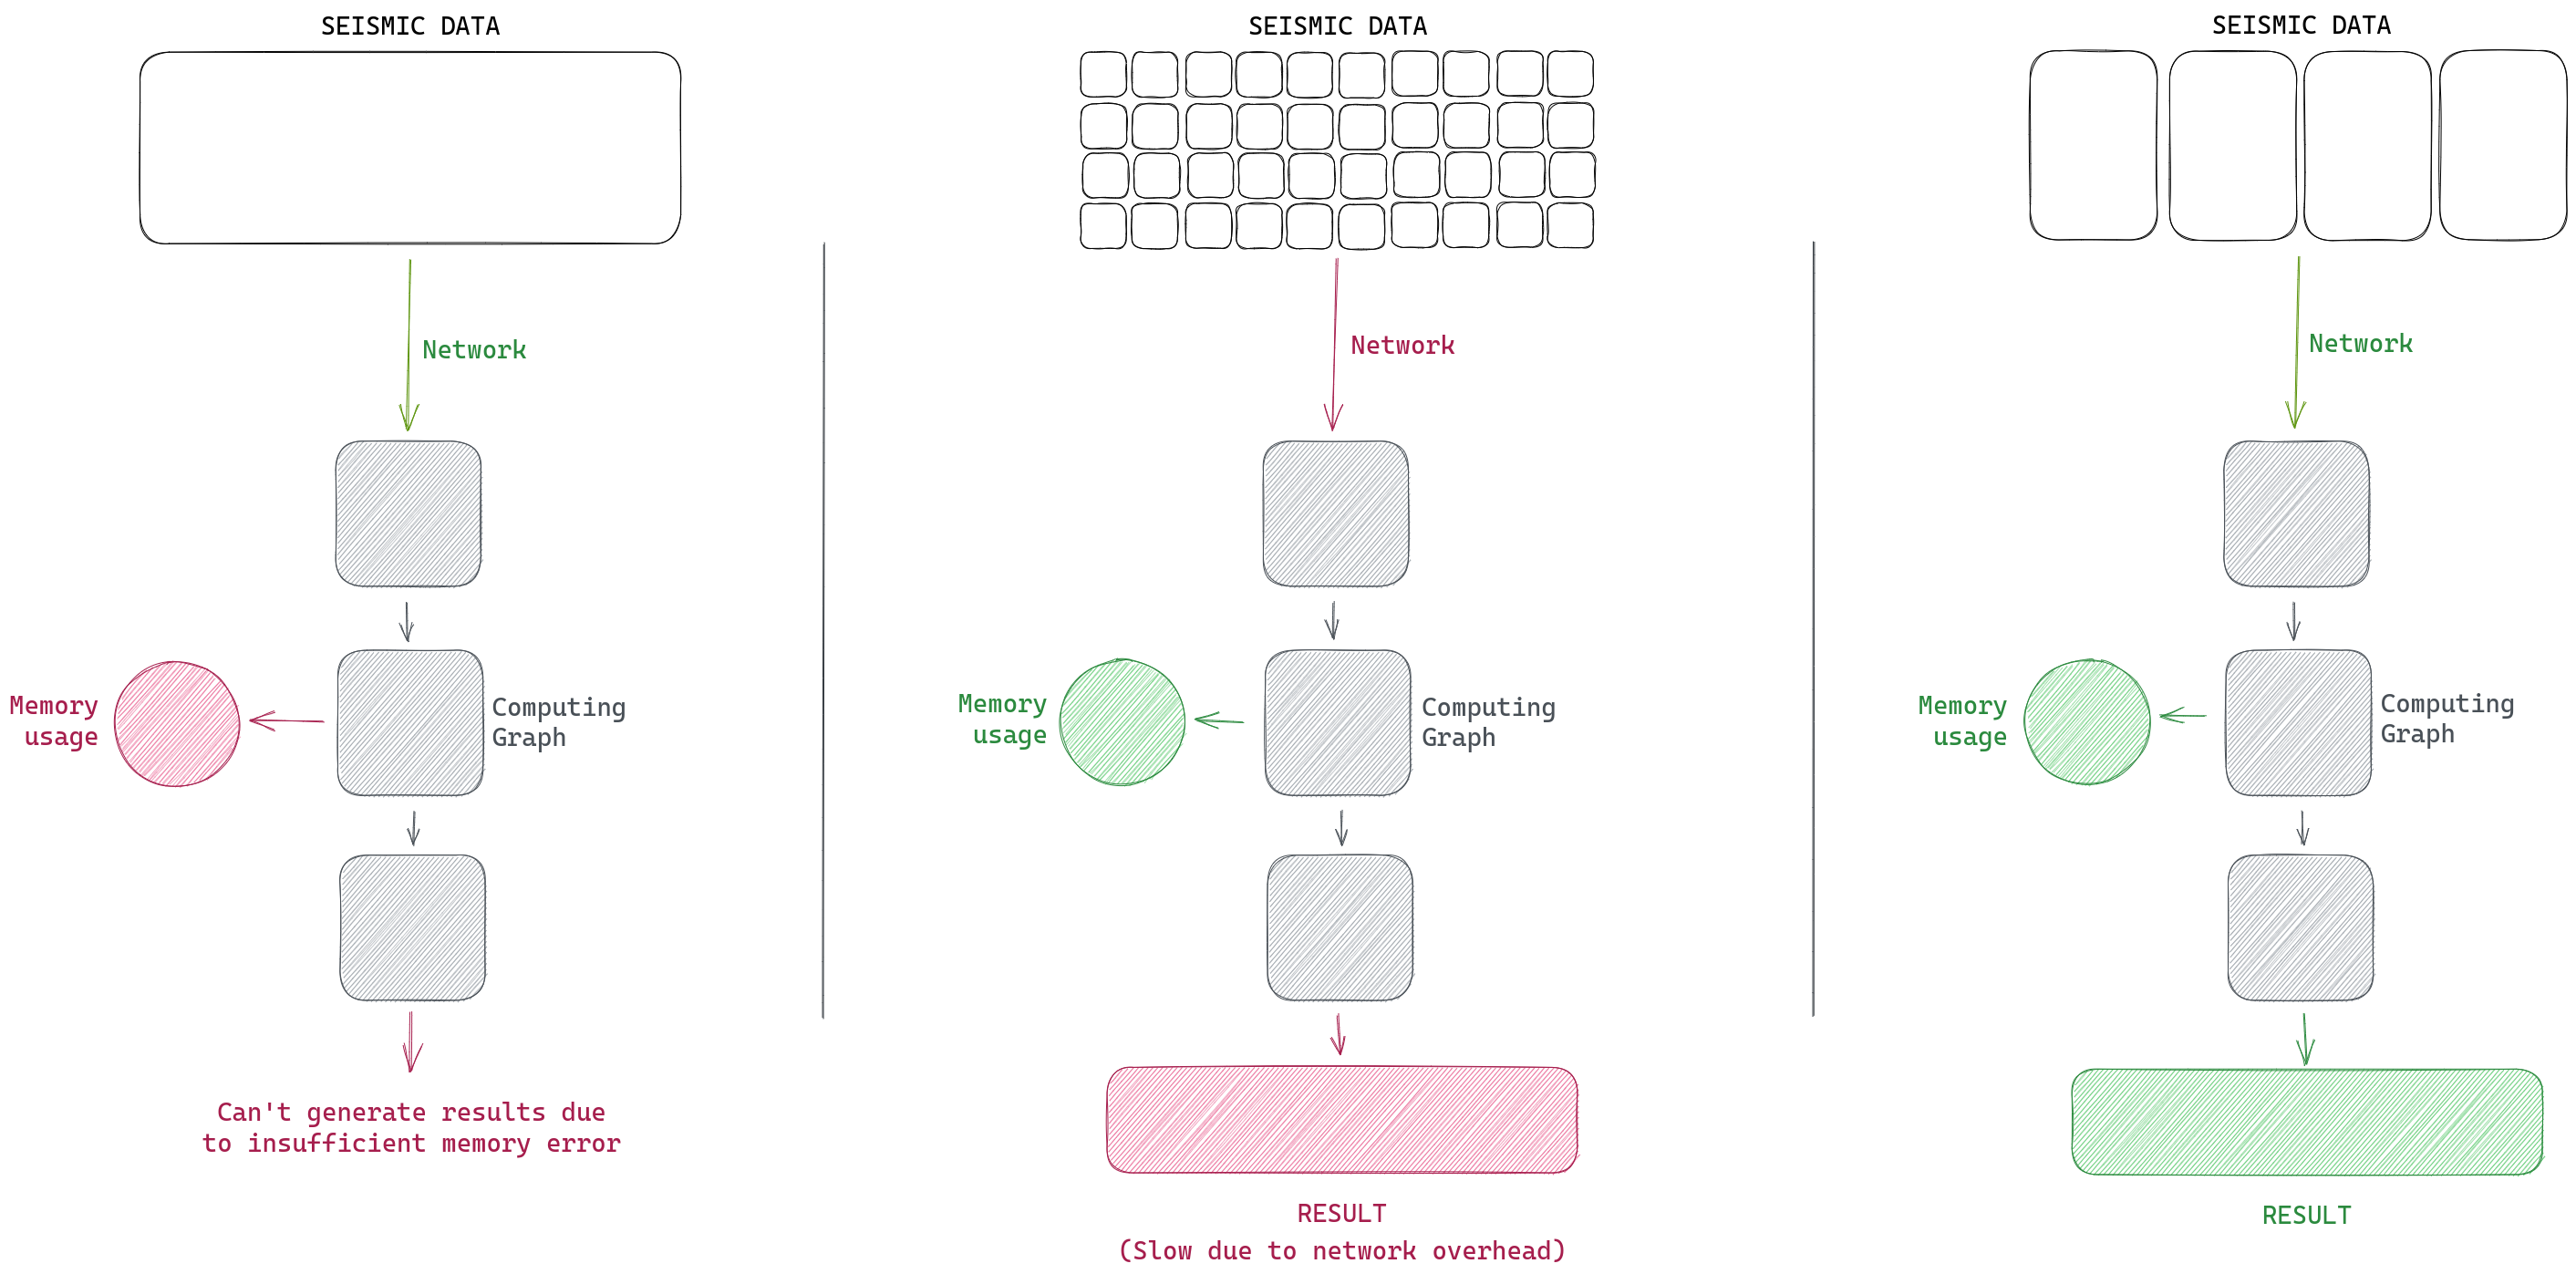
\includegraphics{block_size.png}
  }
\end{figure}

While executing the graph, the developer must manually set the block\_size parameter.
Setting a large number may lead to memory issues and cause significant delays due the trial-and-error nature of the execution flow.
Since Petrobras uses supercomputers to execute those graphs, this delay is even larger considering the time it takes to submit a job due to the queue waiting time.

On the other hand, setting a small number may increase the execution time due to \EBC{network overhead}{Seria bom adicionar referências para trabalhos que mostram que este é o gargalo ou mostrar resultados experimentais onde isso acontece}.
Since Petrobras have a large number of graphs to execute, and each graph usually takes a long time to execute, I need to find a way to optimize the block\_size parameter.

Dask~\cite{dask} provides an automatic chunking feature, but it relies on the chunk\_size parameter, which is a static parameter define prior to execution.
Since the developer do need to define this parameter prior to the execution, they can't rely on Dask~\cite{dask} auto chunking feature to automatically split the data, but they can rely on the automatic chunking if they figure out the ideal chunk\_size prior to the execution.

Figuring out the chunk\_size for algorithms that doesn't require a large working memory is easy, since the developer can set that to a percentage of the available memory.
But, some of the seismic operators used by Petrobras generates a large working memory during the graph execution, which makes it difficult to determine the ideal chunk\_size.

Based on this assumption, if someone predicts the memory usage of the graph that person can use the Dask~\cite{dask} auto chunking feature to automatically split the data into the ideal number of chunks.
Since \ac{DASF}~\cite{dasf} uses Dask~\cite{dask} under the hood, the block\_size parameter on \ac{DASF}~\cite{dasf} is equivalent to the chunk\_size parameter on Dask~\cite{dask}.
Therefore, this research aims to develop an automated data partitioning strategy that is memory-footprint aware.
In other words, I aim to create a \ac{DASF}~\cite{dasf} plugin that can automatically set the optimal block\_size parameter during execution based on a machine learning model that can predict the memory-footprint of the algorithm.
This will help Petrobras to optimize resource utilization and minimize waiting and execution time.
The model will provide a comprehensive understanding of memory usage patterns for different block sizes and contribute to the development of a more efficient data partitioning strategy to execute a graph in large-scale clusters.
